\documentclass{beamer}
\usepackage[utf8]{inputenc}
\usepackage{ifpdf}
%\usepackage{hyperref}
\usepackage[english]{babel}
\usepackage{amsfonts}
\usepackage{amsmath}
\usepackage{amsthm}
\usepackage{color}
\usepackage{graphicx}
\usepackage{tikz}
%\usepackage{multicol}
%\usepackage{moreverb}
\usepackage{listings}
%\usepackage{color}
%\usepackage{algorithm}
%\usepackage{algorithmicx}
%\usepackage{algpseudocode}
%\usepackage{longtable}
%\usepackage{geometry}
%\geometry{margin=2cm}
%\floatname{algorithm}{Algorithmus}
\usepackage{pgfpages}

\usetikzlibrary{decorations.pathmorphing}
\usetikzlibrary{decorations.pathreplacing}
\usetikzlibrary{shapes.callouts}

\title{Collaborative Evaluation of Arbitrary Functions in a Constant Number of Rounds with Polynomial Amount of Communication}
\subtitle{Secure Multiparty Computation}
\author[P. Müller]{Philipp Müller}
\institute[TUM]{Technische Universität München}
\date{July 17, 2012}

\usetheme[compress]{Singapore}
\useinnertheme{rectangles}

\DeclareMathOperator*{\argmax}{arg\,max}

\lstset{
	basicstyle=\ttfamily,
	tabsize=2
}

%\setbeameroption{show notes on second screen=left}

\setbeamertemplate{footline}
{
  \hbox{
    \begin{beamercolorbox}[wd=\paperwidth,ht=0.2cm,dp=0.2cm]{page footer}
      \begin{columns}
        \begin{column}{.33\paperwidth}
          \centering{}
        \end{column}
        \begin{column}{.33\paperwidth}
          \centering{}
          \insertframenumber 
        \end{column}
        \begin{column}{.33\paperwidth}
          \centering
        \end{column}
      \end{columns}
    \end{beamercolorbox}
  }
  \vskip0pt
}
\usenavigationsymbolstemplate{}

\newcommand{\todo}[1]{ {\color{red}{#1} }}

\tikzset{onslide/.code args={<#1>#2}{%
  \only<#1>{\pgfkeysalso{#2}} 
}}

%\usetheme[compress]{Berlin}

\AtBeginPart{
  \begin{frame}
    \partpage
    %\setcounter{tocdepth}{1}
    %\tableofcontents
  \end{frame}
}

\begin{document}

\begin{frame}
  \maketitle{}
\end{frame}

% \begin{frame}
%   \frametitle{Motivation}
%   \begin{itemize}
%   \item Some cryptographers want to know who has the best password
%   \end{itemize}
%   \begin{center}
%     \begin{tikzpicture}[scale=1.2]
%       \draw[white] (0,-1)rectangle(6,2);
%       \foreach \x in {1,2,3,4} {
%       \begin{scope}[xshift=\x cm,scale=0.7,decorate]
%         \draw[decorate,decoration={random steps, segment length=1mm, amplitude=.12mm}] (0,0) circle (.5);
%         \draw[decorate,decoration={random steps, segment length=1mm, amplitude=.12mm}] (0,-.5) -- (0,-1);
%         \draw[decorate,decoration={random steps, segment length=1mm, amplitude=.12mm}] (0,-.7) -- (-.4, -.5);
%         \draw[decorate,decoration={random steps, segment length=1mm, amplitude=.12mm}] (0,-.7) -- (+.4, -.5);
%         \draw[decorate,decoration={random steps, segment length=1mm, amplitude=.12mm}] (0,-1) -- (-.4, -1.2);
%         \draw[decorate,decoration={random steps, segment length=1mm, amplitude=.12mm}] (0,-1) -- (+.4, -1.2);
%       \end{scope}
%     }
%       \begin{scope}[xshift=5 cm,scale=0.7,decorate, yshift=0]
%         \only<-2>{\draw[decorate,decoration={random steps, segment length=1mm, amplitude=.12mm}] (0,0) circle (.5);}
%         \draw[decorate,decoration={random steps, segment length=1mm, amplitude=.12mm}] (0,-.5) -- (0,-1);
%         \draw[decorate,decoration={random steps, segment length=1mm, amplitude=.12mm}] (0,-.7) -- (-.4, -.5);
%         \draw[decorate,decoration={random steps, segment length=1mm, amplitude=.12mm}] (0,-.7) -- (+.4, -.5);
%         \draw[decorate,decoration={random steps, segment length=1mm, amplitude=.12mm}] (0,-1) -- (-.4, -1.2);
%         \draw[decorate,decoration={random steps, segment length=1mm, amplitude=.12mm}] (0,-1) -- (+.4, -1.2);
%         \only<2>{
%         \node[rounded corners, rectangle callout, callout relative pointer=(315:.5cm), draw=black, text width=4.8cm, decorate, decoration={random steps, segment length=1mm, amplitude=.12mm}] at (-1.8,1.8) {``Well, you could all give me your passwords, and I'll tell you who had the best one!''};
%       }
%         \only<3>{
%         \node at (0,0) {\includegraphics[scale=0.08]{troll.png}};
%       }
%       \end{scope}
%     \end{tikzpicture}
%   \end{center}
% \end{frame}

\part{A short introduction to collaborative secure function evaluation}
\label{part:mainpart}

\section{Setting}
\label{sec:setting}

\subsection{Our Problem}

\begin{frame}
  \frametitle{A motivational problem}  
  \begin{itemize}
  \item Several firms (numbered 1 to $n$) want to buy another firm
  \item Best bid wins!
  \item Participants only want to know \emph{who} has best bid, \emph{not how high} it was
  \item Mathematical formulation: 
    \begin{equation*}
      \argmax_{i\in\left\{ 1,2,\dots,n \right\}} \left\{ x_i \mid x_i \text{ is bid of firm } i \in \left\{ 1,2,\dots,n \right\} \right\}
    \end{equation*}

  \end{itemize}
\end{frame}

\begin{frame}
  \frametitle{Problem}  
  \note[item]{ No third party!}
  \begin{itemize}
  \item Function accepting some arguments
  \item Each argument supplied by another party\footnote{Also called player, participant.}
  \item Goal: Function evaluation, but keep arguments secret
    \note[item]{Secret with respect to the output!}
  \item Possibly dishonest participants
  \end{itemize}
  \begin{example}
    \begin{equation}
      \label{eq:example-function}
      f(x,y,z) = (x\wedge y)\vee z
    \end{equation}
  \end{example}
\end{frame}

\subsection{Functions as Circuits}

% \begin{frame}
%   \frametitle{Functions as circuits}
%   \begin{itemize}
%   \item Idea: Represent functions as circuits
%   \item Restrictions:
%     \begin{itemize}
%     \item No cycles
%     \item Only 2/1- or 1/2-gates
%     \end{itemize}

%   \end{itemize}
  
%   \begin{center}
%     \begin{tikzpicture}
%       \node(AND) at (0,1) [rectangle,draw=black] {AND}; \node (OR) at
%       (.5,2) [rectangle,draw=black] {OR}; \draw[<-,semithick]
%       (-.2,.75) |- +(-.4,-.4) -- +(-.4,-.8) node[below] {$x$};
%       \draw[<-,semithick] (.2,.75) |- +(+.3,-.4) -- +(+.3,-.8)
%       node[below] {$y$}; \draw[<-,semithick] (0.35,1.75) -- +(0,-.3)
%       -| (AND); \draw[<-,semithick] (0.65,1.75) -- +(0,-.3) -|
%       +(.7,-1.8) node[below] {$z$}; \draw[->,semithick] (OR) --
%       +(0,0.6) node[above] {$f(x,y,z)$};
%     \end{tikzpicture}
%   \end{center}
% \end{frame}

\begin{frame}
  \frametitle{Functions as circuits}
  \note[item]{Uniform representation!}
  \note[item]{Evaluation}
  Idea: Represent functions as circuits
  \begin{center}
    \begin{tikzpicture}[yshift=-2cm]
      \draw[opacity=0](-1.5,-1.) rectangle (2,4.5);
      \node(AND) at (0,1) [rectangle,draw=black] {AND}; 
      \node (OR) at (.5,3) [rectangle,draw=black] {OR}; 
      \draw[<-,semithick] (-.2,.75) |- +(-.4,-.4) -- +(-.4,-.8) node[below] {$x$\only<2->{=0}};
      \draw[<-,semithick] (.2,.75) |- +(+.3,-.4) -- +(+.3,-.8) node[below] {$y$\only<2->{=1}}; 
      \draw[<-,semithick] (0.35,2.75) -- +(0,-.3) -| node[left]{\only<3->{0}} (AND); 
      \draw[<-,semithick] (0.65,2.75) -- +(0,-.3) -| +(.7,-2.8) node[below] {$z$\only<2->{=1}}; 
      \draw[->,semithick] (OR) -- +(0,0.6) node[above] {$f(x,y,z)$\only<4->{=1}};
    \end{tikzpicture}
  \end{center}
\end{frame}

\begin{frame}
  \frametitle{Problem}
  \note{``When we see a 0, it \emph{means} $\mathbf{0}$''}
  \note[item]{But: Computation must stay correct}
  \begin{itemize}
  \item ``If we write a 0, it represents 0!''
  \item Each player can see/deduce everything
  \item Idea: ``Ensure that each player sees some (random) stuff, but can't decide whether it's a 0 or a 1''

    $\Rightarrow$ Distinguish between \emph{signals} and \emph{plain-text}\footnote{The plain-text is also called \emph{semantics}, but I (try to) use the term plain-text since the term semantics is later used for something else.}

    $\Rightarrow$ Basic idea behind ``garbled circuits''
  \end{itemize}
\end{frame}

% \section{Idea: Garbled Circuits}
% \label{sec:solution-garbled-circuits}

\subsection{Hiding Semantics}

\begin{frame}
  \frametitle{Garbled circuits -- overview}
  \begin{itemize}
    \note{These signals are not published. This is just the idea!}
  \item Up to now: Signal 0 means plain-text $\mathbf{0}$, signal 1 means $\mathbf{1}$
  \item Garbled circuit: Assign random signals to each wire!
  \item<alert@2> Idea: Hide plain-text by assigning random signals 
  \end{itemize}

  \begin{center}
    \begin{tikzpicture}
      % auxiliary
      \draw[white](-3,-1)rectangle(5,4.5);
      % now onto the real stuff
      \node (AND) at (0,1) [rectangle,draw=black] {AND};
      \node (OR) at (1,3) [rectangle,draw=black] {OR};
      % x->AND
      \draw[<-,semithick] (-.2,.75) |- +(-.5,-.4) -- 
      node[yshift=2mm,left] {\only<1>{0 }\only<2>{1110 }$\leftrightarrow \mathbf{0}$} 
      node[yshift=-2mm,left] {\only<1>{1 }\only<2>{0101 }$\leftrightarrow \mathbf{1}$} 
      +(-.5,-1.2) node[below] {$x$};
      % y->AND
      \draw[<-,semithick] (.2,.75) |- +(+.3,-.4) -- 
      node[yshift=2mm,right] {\only<1>{0 }\only<2>{1001 }$\leftrightarrow \mathbf{0}$} 
      node[yshift=-2mm,right] {\only<1>{1 }\only<2>{1010 }$\leftrightarrow \mathbf{1}$} 
      +(+.3,-1.2) node[below] {$y$};
      % AND->OR
      \draw[<-,semithick] (.8,2.75) |- +(-.8,-.5) 
      node[yshift=2mm,left] {\only<1>{0 }\only<2>{0011 }$\leftrightarrow \mathbf{0}$ }
      node[yshift=-2mm,left] {\only<1>{1 }\only<2>{1010 }$\leftrightarrow \mathbf{1}$ } --
      (AND);
      % z->OR
      \draw[<-,semithick] (1.2,2.75) |- ++(+1.4,-.5) 
      node[yshift=2mm,right] {\only<1>{0 }\only<2>{0111 }$\leftrightarrow \mathbf{0}$} 
      node[yshift=-2mm,right] {\only<1>{1 }\only<2>{1000 }$\leftrightarrow \mathbf{1}$} --
      +(0,-2.7) node[below] {$z$};
      % OR->output
      \draw[->,semithick] (OR) -- 
      node[yshift=2mm,right] {\only<1>{0 }\only<2>{0010 }$\leftrightarrow \mathbf{0}$} 
      node[yshift=-2mm,right] {\only<1>{1 }\only<2>{1011 }$\leftrightarrow \mathbf{1}$} 
      +(0,1.4);
    \end{tikzpicture}
  \end{center}
\end{frame}

% \subsection{Some Words on Garbled Signals}

\begin{frame}
  \frametitle{Garbled circuit -- signals and plain-text}
  \begin{columns}
    \begin{column}{.6\textwidth}
      \begin{itemize}
        \note{Each wire can hold two values $\Rightarrow$ we need two signals per wire}
      \item \emph{Odd} and \emph{even} signals for each wire (``parity'')
      \item One of those represents plain-text $\mathbf{0}$, the other plain-text $\mathbf{1}$
      \item Signals and mapping chosen randomly by all players
      \item<alert@2> Special case output wires: Even signal means
        $\mathbf{0}$, odd means $\mathbf{1}$
      \end{itemize}
    \end{column}

    \begin{column}{.4\textwidth}
      \begin{center}
        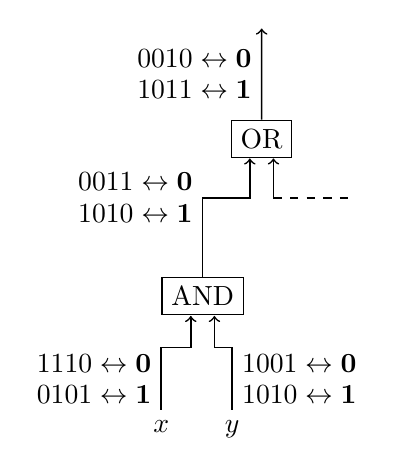
\begin{tikzpicture}[xscale=.75,yscale=1]
          \node (AND) at (0,1) [rectangle,draw=black] {AND}; \node
          (OR) at (1,3) [rectangle,draw=black] {OR};
          % x->AND
          \draw[<-,semithick] (-.2,.75) |- +(-.5,-.4) --
          node[yshift=2mm,left] {$1110\leftrightarrow \mathbf{0}$}
          node[yshift=-2mm,left] {$0101\leftrightarrow \mathbf{1}$}
          +(-.5,-1.2) node[below] {$x$};
          % y->AND
          \draw[<-,semithick] (.2,.75) |- +(+.3,-.4) --
          node[yshift=2mm,right] {$1001\leftrightarrow \mathbf{0}$}
          node[yshift=-2mm,right] {$1010\leftrightarrow \mathbf{1}$}
          +(+.3,-1.2) node[below] {$y$};
          % AND->OR
          \draw[<-,semithick] (.8,2.75) |- +(-.8,-.5)
          node[yshift=2mm,left] {$0011\leftrightarrow \mathbf{0}$ }
          node[yshift=-2mm,left] {$1010\leftrightarrow \mathbf{1}$ }
          -- (AND);
          % z->OR
          % \draw[<-,semithick] (1.2,2.75) |- ++(+1.4,-.5)
          % node[yshift=2mm,right] {$0111\leftrightarrow \mathbf{0}$}
          % node[yshift=-2mm,right] {$1000\leftrightarrow \mathbf{1}$}
          % --
          % +(0,-2.7) node[below] {$z$};
          \draw[<-,semithick] (1.2,2.75) -- ++(0,-.5);
          \draw[dashed,semithick] (1.2,2.75) ++(0,-.5) -- ++(1.4,0);
          % OR->output
          \draw[->,semithick] (OR) -- node[yshift=2mm,left,onslide=<2>{red}]
          {$0010\leftrightarrow \mathbf{0}$} node[yshift=-2mm,left,onslide=<2>{red}]
          {$1011\leftrightarrow \mathbf{1}$} +(0,1.4);
        \end{tikzpicture}
      \end{center}
    \end{column}
  \end{columns}

\end{frame}

% \subsection{Our Goal}

\begin{frame}
  \frametitle{Our ultimate goal}
  \setbeamercovered{transparent}
  \begin{itemize}
    \note[item]{Players shall only receive a circuit and the garbled input signals associated with proper input bits.}
    \note[item]{Show input bits}
    \note[item]{show garbled input signals}
    \note[item]{show computed garbled signals}
    \note[item]{hide other signals, even semantics}
    \note[item]{this is all}
  \item Compute \emph{correct} output given only garbled circuit with inputs
  \item<6-> Everything else shall stay unknown\only<8->{, even the semantics}
  \item<10-> This is everything a player should see
  \end{itemize}

  \begin{center}
    \begin{tikzpicture}
      % auxiliary
      \draw[white](-3,-1.6)rectangle(5,4.5);
      % now onto the real stuff
      \node (AND) at (0,1) [rectangle,draw=black] {AND};
      \node (OR) at (1,3) [rectangle,draw=black] {OR};
      % x->AND
      \draw[<-,semithick] (-.2,.75) |- +(-.5,-.4) -- 
      node[yshift=2mm,left,opacity=0.3,onslide=<3->{opacity=1}] {1110 \only<-8>{\only<3->{\color{black!30!white}}{$\leftrightarrow \mathbf{0}$}}}
      node[yshift=-2mm,left,opacity=0.3,onslide=<7->{opacity=0}] {$0101 \leftrightarrow \mathbf{1}$} 
      +(-.5,-1.2) node[below] {$x$\only<2>{=0}};
      % y->AND
      \draw[<-,semithick] (.2,.75) |- +(+.3,-.4) -- 
      node[yshift=2mm,right,opacity=0.3,onslide=<7->{opacity=0}] {$1001 \leftrightarrow \mathbf{0}$} 
      node[yshift=-2mm,right,opacity=0.3,onslide=<3->{opacity=1}] {1010 \only<-8>{\only<3->{\color{black!30!white}}{$\leftrightarrow \mathbf{1}$}}} 
      +(+.3,-1.2) node[below] {$y$\only<2>{=1}};
      % AND->OR
      \draw[<-,semithick] (.8,2.75) |- +(-.8,-.5) 
      node[yshift=2mm,left,opacity=0.3,onslide=<4->{green!40!black,opacity=1}] {0011 \only<-8>{\only<4->{\color{black!30!white}}{$\leftrightarrow \mathbf{0}$}} }
      node[yshift=-2mm,left,opacity=0.3,onslide=<7->{opacity=0}] {$1010 \leftrightarrow \mathbf{1}$ } --
      (AND);
      % z->OR
      \draw[<-,semithick] (1.2,2.75) |- ++(+1.4,-.5) 
      node[yshift=2mm,right,opacity=0.3,onslide=<7->{opacity=0}] {$0111 \leftrightarrow \mathbf{0}$} 
      node[yshift=-2mm,right,opacity=0.3,onslide=<3->{opacity=1}] {1000 \only<-8>{\only<3->{\color{black!30!white}}{$\leftrightarrow \mathbf{1}$}}} --
      +(0,-2.7) node[below] {$z$\only<2>{=1}};
      % OR->output
      \draw[->,semithick] (OR) -- 
      node[yshift=2mm,right,opacity=0.3,onslide=<7->{opacity=0}] {$0010 \leftrightarrow \mathbf{0}$} 
      node[yshift=-2mm,right,opacity=0.3,onslide=<5->{green!40!black,opacity=1}] {$1011\leftrightarrow \mathbf{1}$} 
      +(0,1.4);
    \end{tikzpicture}
  \end{center}
\end{frame}

\begin{frame}
  \frametitle{Our ultimate goal -- outlook}
  
  \begin{center}
    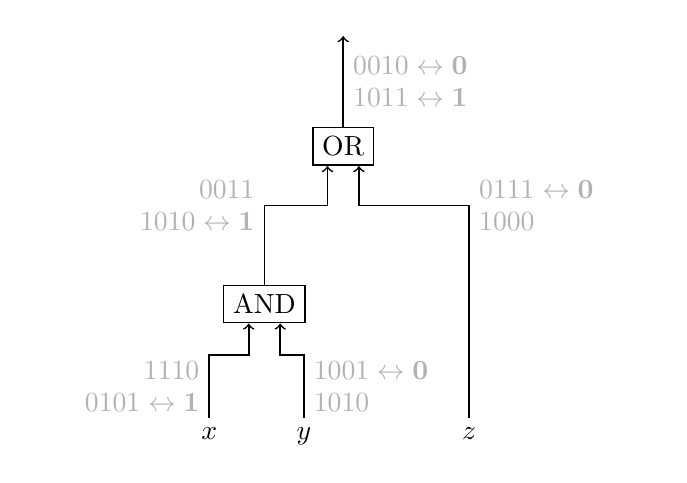
\begin{tikzpicture}
      % auxiliary
      \draw[white](-3,-0.9)rectangle(5,4.5);
      % now onto the real stuff
      \node (AND) at (0,1) [rectangle,draw=black] {AND};
      \node (OR) at (1,3) [rectangle,draw=black] {OR};
      % x->AND
      \draw[<-,semithick] (-.2,.75) |- +(-.5,-.4) -- 
      node[yshift=2mm,left,opacity=0.3,onslide=<1->{opacity=1}] {1110}
      node[yshift=-2mm,left,opacity=0.3,onslide=<1->{opacity=0}] {$0101 \leftrightarrow \mathbf{1}$} 
      +(-.5,-1.2) node[below] {$x$};
      % y->AND
      \draw[<-,semithick] (.2,.75) |- +(+.3,-.4) -- 
      node[yshift=2mm,right,opacity=0.3,onslide=<1->{opacity=0}] {$1001 \leftrightarrow \mathbf{0}$} 
      node[yshift=-2mm,right,opacity=0.3,onslide=<1->{opacity=1}] {1010 } 
      +(+.3,-1.2) node[below] {$y$};
      % AND->OR
      \draw[<-,semithick] (.8,2.75) |- +(-.8,-.5) 
      node[yshift=2mm,left,opacity=0.3,onslide=<1->{green!40!black,opacity=1}] {0011 }
      node[yshift=-2mm,left,opacity=0.3,onslide=<1->{opacity=0}] {$1010 \leftrightarrow \mathbf{1}$ } --
      (AND);
      % z->OR
      \draw[<-,semithick] (1.2,2.75) |- ++(+1.4,-.5) 
      node[yshift=2mm,right,opacity=0.3,onslide=<1->{opacity=0}] {$0111 \leftrightarrow \mathbf{0}$} 
      node[yshift=-2mm,right,opacity=0.3,onslide=<1->{opacity=1}] {1000 } --
      +(0,-2.7) node[below] {$z$};
      % OR->output
      \draw[->,semithick] (OR) -- 
      node[yshift=2mm,right,opacity=0.3,onslide=<1->{opacity=0}] {$0010 \leftrightarrow \mathbf{0}$} 
      node[yshift=-2mm,right,opacity=0.3,onslide=<1->{green!40!black,opacity=1}] {$1011\leftrightarrow \mathbf{1}$} 
      +(0,1.4);
    \end{tikzpicture}
  \end{center}
  \begin{itemize}
  \item How to compute the signals?
  \item How to map from signals onto meanings?
  \item How to ``implement'' gates?
  \end{itemize}
\end{frame}

\section{Prerequisites}
\label{sec:prerequisites}

% \subsection{Protocols}
% \label{sec:protocols-definition}

% \begin{frame}
%   \frametitle{What is a protocol?}
%   \begin{itemize}
%   \item Each participant has to conform some rules
%   \item Usually organized in rounds
%   \item May work even with malicious players (\emph{adversaries})
%   \item Complexity measure: Rounds and communication
%   \end{itemize}
%   % \begin{exampleblock}{Simple (insecure) protocol to flip a coin}
%   %   \begin{itemize}
%   %   \item Each player randomly tosses a coin to get a random number in $\{0,1\}$
%   %   \item Players reveal their numbers\dots
%   %   \item \dots and compute the XOR of the numbers
%   %   \end{itemize}
%   %   \note[item]{Protocol of course insecure, but working if at least one single player is honest.}
%   %   \note[item] {Rounds is the limiting resource.}
%   % \end{exampleblock}
% \end{frame}

\subsection{Model of Computation}
\label{sec:model-of-computation}

\begin{frame}
  \frametitle{Model of computation -- protocols}
  \begin{itemize}
  \item Network of $n$ players
  \item Private channels and broadcast channel
  \item Access to a fair coin
  \item Local computation ``instant'', communication expensive
  \end{itemize}
  Protocol:
  \begin{itemize}
  \item Certain ``rules'' for each player
  \item Organized in rounds
  \item May work in presence of malicious players (\emph{adversaries})
  \item Complexity measure: Rounds and communication
    
    $\Rightarrow$ Rounds are the limiting resource
    \note[item]{Remember that rounds/communication was mentioned in the title.}
  \end{itemize}
\end{frame}

\subsection{Adversaries}
\label{sec:adversaries}

\begin{frame}
  \frametitle{Adversaries}
  \begin{itemize}
  \item \emph{One single} adversary\dots
  \item \dots that can infect several players
  \item Adversary can infect players at the beginning of each round as he wishes
  \item Adversary controls infected players fully
  \item Can infect less than half of the players
    \note{Adversaries leave Honest majority}
  \end{itemize}
\end{frame}

\begin{frame}
  \frametitle{Our notion of security}
  Protocol shall:
  \begin{itemize}
  \item yield \emph{correct} result in the presence of up to $\lfloor (n-1)/2 \rfloor$ dishonest participants
  \item compute the result securely (inputs shall not become public)
  \item not enable the adversary to deduce inputs.
  \end{itemize}

\end{frame}

\subsection{Pseudorandom Generators}
\label{sec:pseudorandom-generators}

\begin{frame}
  \frametitle{Pseudorandom generators}
  \begin{itemize}
  \item Deterministic, poly-time algorithm
  \item Takes a (truly random) string and stretches it to a longer string
  \item Output \emph{indistinguishable} from truly random source
  \item Pseudorandom generators are one-way!
  \end{itemize}
\end{frame}

% \begin{frame} % alte pg-slide
%   \frametitle{Pseudorandom Generators $G_0$ and $G_1$}
%   \note[item]{Table note for $G_0$ and $G_1$.}
%   \begin{itemize}
%   \item Input: Binary string of length $k$
%   \item Output: Binary string of length $2\overline{n}k+2$, where $\overline{n}=k^{10}$
%   \item Number of players bounded by $\overline{n}$
%     % \item More formal: $G: \Sigma^{k} \rightarrow \Sigma^{2\overline{n}k+2}$
%   \end{itemize}
%   \begin{center}
%     \begin{tikzpicture}
%       \draw[opacity=0](1,-2) rectangle (10,2);
%       \node[draw,rectangle,minimum height=.7cm](i) at (1,1) {$s$};
%       \node[draw,rectangle,minimum height=.7cm,minimum width=4cm](o0) at (4,1) {
%         % $G'_0(s)$
%       };
%       \node[draw,rectangle,minimum height=.7cm,minimum width=4cm](o1) at (8,1) {
%         % $G'_1(s)$
%       };
%       \draw[semithick,->] (i) -- node[above]{$G$} (o0);
%       \draw[decorate,decoration=brace] (2.1,1.5) -- node[above]{$\overline{n}k+1$ bits}(5.9,1.5);
%       \draw[decorate,decoration=brace] (6.1,1.5) -- node[above]{$\overline{n}k+1$ bits}(9.9,1.5);
%       \only<2-> {
%         \draw[decorate,decoration=brace,text width=2cm] (4.5,0.5) -- node[below]{$nk+1$ bits}(2.1,0.5);
%         \draw[decorate,decoration=brace,text width=2cm] (8.5,0.5) -- node[below]{$nk+1$ bits}(6.1,0.5);
%         \draw[semithick,dashed](4.5,0.5)--(4.5,1.5);
%         \draw[semithick,dashed](8.5,0.5)--(8.5,1.5);
%         \node[minimum width=2.5cm] at (3.25, 1) {$G_0(s)$};
%         \node[minimum width=2.5cm] at (7.25, 1) {$G_1(s)$};
%         \draw[->,semithick](5.3,-1.25) .. controls +(-.0,.25) and +(0,-.5) .. (3.5,-.15);
%         \draw[->,semithick](5.8,-1.25) .. controls +(-.0,.25) and +(0,-.5) .. (7.5,-.15);
%         \node at (5.7, -1.5) {Will be used later};
%       }
%     \end{tikzpicture}
%   \end{center}
%   $\Rightarrow$ \alert<3>{$G_{\{0,1\}}: \{0,1\}^k\rightarrow \{0,1 \}^{nk+1}$}, with:
%   \begin{itemize}
%   \item $n$: Number of players
%   \item $k$: Security parameter
%   \end{itemize}
% \end{frame}

\begin{frame}
  \frametitle{Pseudorandom generators $G_0$ and $G_1$}
  \note[item]{Table note for $G_0$ and $G_1$.}
  \begin{itemize}
  \item Input: Binary string of length $k$
  \item Output: Binary string of length $\overline{n}k+1$, where $\overline{n}=k^{10}$
  \item Number of players bounded by $\overline{n}$
    % \item More formal: $G: \Sigma^{k} \rightarrow \Sigma^{2\overline{n}k+2}$
  \item $\Rightarrow$ \alert<2>{$G_{\{0,1\}}: \{0,1\}^k\rightarrow \{0,1 \}^{nk+1}$}, with:
    \begin{itemize}
    \item $n$: Number of players
    \item $k$: Security parameter
    \end{itemize}
  \item $G_0$ and $G_1$ are independent of each other
  \end{itemize}
\end{frame}

\subsection{Computing on Shared Bits}
\label{sec:computing-on-shared-bits}

\begin{frame}
  \frametitle{Our basic building blocks}
  \note[item] {This problem has been subject to research, so there are some protocols that have been proven.}
  \note[item] {But these work only for particular functions. }
  \note[item] {Of course, we cannot use these protocols to directly evaluate our (possibly very complicated) circuit, but we will use them as base.}
  \note[item] {Remind that no. of rounds/poly-communication was stated as goal in the title.}
  There are protocols to
  \begin{itemize}    
  \item<alert@2> compute the XOR (denoted by the symbol $\oplus$) of an arbitrary number of bits
  \item<alert@2> evalutate any circuit of constant depth with bounded fan-in
  \end{itemize}
  in a constant number of rounds with polynomial\footnote{W.r.t. circuit size and $k$} communication.
  
  Proven secure for honest majority.
\end{frame}

\part{The protocol}
\label{part:the-protocol}

\section{Overview}
\label{sec:implementing-the-protocol}

\subsection{Three Phases of the Protocol}
\label{sec:two-phases-of-protocol}

\begin{frame}
  \frametitle{Three phases in the protocol}
  \begin{enumerate}
    \setcounter{enumi}{-1}
  \item Preprocessing: Bring circuit in particular form
  \item Players collaboratively compute garbled circuit and garbled input signals
  \item Players locally evaluate garbled circuit on garbled input signals
  \end{enumerate}
  % \begin{alertblock}{Remark}
  %   Local evaluation cheap, while collaborative computation of the circuit is the expensive thing.
  % \end{alertblock}
  \note[item] {Local evaluation cheap, collborative construction expensive.}
\end{frame}

\subsection{Phase 0: Bringing the circuit into a suitable format}
\label{sec:circuit-suitable-format}

\begin{frame}
  \frametitle{Phase 0: suitable format of the circuit}
  \begin{enumerate}
    \setcounter{enumi}{-1}
  \item No cycles, only gates of types AND, XOR, NEG, OR
  \item Convert all gates to 2/1-gates $\Rightarrow$ ``binary tree construction''
    \begin{center}
      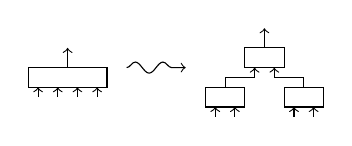
\begin{tikzpicture}[draw=black,scale=.25]
        \draw[](0,0) rectangle (4,1);
        \draw[->] ( .5,-.5) -- ( .5,0);
        \draw[->] (1.5,-.5) -- (1.5,0);
        \draw[->] (2.5,-.5) -- (2.5,0);
        \draw[->] (3.5,-.5) -- (3.5,0);
        \draw[->] (2,1) -- (2,2);
        \draw[->,decorate,decoration={snake,amplitude=2,post length=2}] (5,1) -- (8,1);
        % bintree
        \begin{scope}[xshift=9cm,yshift=-1cm]
          \draw(0,0) rectangle (2,1);
          \draw(4,0) rectangle (6,1);
          \draw(2,2) rectangle (4,3);
          \draw[->] ( .5,-.5) -- ( .5,0);
          \draw[->] (1.5,-.5) -- (1.5,0);
          \draw[->] (4.5,-.5) -- (4.5,0);
          \draw[->] (5.5,-.5) -- (5.5,0);
          \draw[->] (1,1) -- (1,1.5) -| (2.5,2);
          \draw[->] (5,1) -- (5,1.5) -| (3.5,2);
          \draw[->] (3,3) -| (3,4);
        \end{scope}
      \end{tikzpicture}
    \end{center}
  \item Each wire is used as input wire \emph{at most once} $\Rightarrow$ introduce ``splitters''
    \begin{center}
      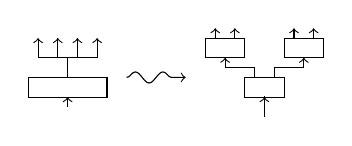
\begin{tikzpicture} [draw=black,scale=.25]
        \draw[](0,0) rectangle (4,1);
        \draw(2,1) -- (2,2);
        \draw[->] (2,2) -| ( .5,3);
        \draw[->] (2,2) -| (1.5,3);
        \draw[->] (2,2) -| (2.5,3);
        \draw[->] (2,2) -| (3.5,3);
        \draw[->] (2,-.5) -- (2,0);
        \draw[->,decorate,decoration={snake,amplitude=2,post length=2}] (5,1) -- (8,1);
        % splitters
        \begin{scope}[xshift=9cm,yshift=3cm,yscale=-1]
          \draw(0,0) rectangle (2,1);
          \draw(4,0) rectangle (6,1);
          \draw(2,2) rectangle (4,3);
          \draw[<-] ( .5,-.5) -- ( .5,0);
          \draw[<-] (1.5,-.5) -- (1.5,0);
          \draw[<-] (4.5,-.5) -- (4.5,0);
          \draw[<-] (5.5,-.5) -- (5.5,0);
          \draw[<-] (1,1) -- (1,1.5) -| (2.5,2);
          \draw[<-] (5,1) -- (5,1.5) -| (3.5,2);
          \draw[<-] (3,3) -| (3,4);
        \end{scope}
      \end{tikzpicture}
    \end{center}
  \end{enumerate}
  \begin{block}{Remark}
    This increases the circuit's size \emph{only} by a polynomial factor.
  \end{block}
\end{frame}

\section{Phase 1}
\label{sec:computing-the-garbled-circuit}

\subsection{Defining signals and semantics}

\begin{frame}
  \frametitle{Defining signals and semantics}
  \begin{itemize}
  \item All players shall contribute to signals and semantics!
  \item Each player $i$ generates the following:
    \begin{itemize}
    \item For each wire $\omega$, two random strings of length $k$: $s_{0,i}^\omega$ and  $s_{1,i}^\omega$
    \item For each wire $\omega$ except output wires, a random bit $\lambda^\omega_i$
    \end{itemize}
  \end{itemize}
  \begin{alertblock}{Remember:}
      Each wire shall obtain an even and an odd signal, that shall be randomly mapped onto $\{0,1\}$ (mapping except for output wires).
  \end{alertblock}
\end{frame}

\begin{frame}
  \frametitle{Signals and semantics -- definition}
  \begin{description}
  \item[The $k$-bit string $s_{p,i}^\omega$] will be the contribution of player $i$ to the \emph{signal} of parity $p$ for wire $\omega$
  \item[The single bit $\lambda^\omega_i$] is the contribution of player $i$ to the \emph{semantics} of wire $\omega$
  \end{description}
  \begin{block}{More precisely:}
    \begin{description}
    \item[Parity $p$ signal for wire $\omega$:] 
      $s_p^\omega := 
      s_{p,1}^\omega \; s_{p,2}^\omega \; \dots \; s_{p,n-1}^\omega \; s_{p,n}^\omega \; p$

      $\Rightarrow$ Lenght of signals: $nk+1$
    \item[Semantics of wire $\omega$:] 
      $\lambda^\omega := 
      \lambda_1^\omega \, \oplus \, \lambda_2^\omega \, \oplus \, \dots \, \oplus \, \lambda_{n-1}^\omega \, \oplus \, \lambda_n^\omega$
    \end{description}
  \end{block}
  \begin{alertblock}{Remark}
    These are just \emph{definitions}.
    \note[item]{These definitions define the whole circuit wires, but we will not compute them all! We will just ``exploit'' the definition.}
  \end{alertblock}
\end{frame}

\begin{frame}
  \frametitle{Random signals and semantics -- example}
  Three players and their random strings of length $k=3$:
  \begin{center}
    \begin{tabular}[h]{lccc}
      Player & $P1$ & $P2$ & $P3$ \\
      \hline
      Contribution to $s_0^\omega$ & 100 & 011 & 111 \\
      Contribution to $s_1^\omega$ & 010 & 101 & 001 \\
      Contribution to $\lambda^\omega$ & 0 & 0 & 1
    \end{tabular}
  \end{center}
  Thus:
  \begin{itemize}
  \item $s_0^\omega = 100\,011\,111\,0$
  \item $s_1^\omega = 010\,101\,001\,1$
  \item $\lambda^\omega = 0 \oplus 0 \oplus 1 = 1$
  \end{itemize}
  $\lambda^\omega=1$ means that $s_0^\omega \leftrightarrow \mathbf{1}$ and $s_1^\omega \leftrightarrow \mathbf{0}$
  \note[item]{Tell that this is defined for \emph{every} wire!}
\end{frame}

\begin{frame}
  \frametitle{Things to keep in mind}
  \begin{itemize}
  \item Each wire ``gets'' two signals $s_0^\omega$ and $s_1^\omega$
    \begin{itemize}
    \item Even and odd parity
    \item One of them represents plaintext \textbf{0}, the other one \textbf{1}
    \end{itemize}
  \item Signals and semantics are randomly constructed by all players.
  \item<alert@2> $s_p^\omega$ is the parity-$p$-signal for wire $\omega$
  \item<alert@2> $\lambda^\omega$ is the \emph{semantics} for wire $\omega$
  \item<alert@2> Plain-text bit $b$ on wire $\omega$ $\Rightarrow$ choose signal with parity $b\oplus\lambda^\omega$, i.e. $s^\omega_{(b\oplus\lambda^\omega)}$
    \note[item]{Alert at last three bullet points!}
  \end{itemize}
\end{frame}

\begin{frame}
  \frametitle{A word on semantics}
  \begin{itemize}
  \item $\lambda^\omega=0\Leftrightarrow$ parity $=$ plain-text
  \item $\lambda^\omega=1\Leftrightarrow$ parity $=1-$ plain-text
  \end{itemize}
  \begin{exampleblock}{Example}
    \centering{}
    \begin{tikzpicture}
      \draw[use as bounding box,opacity=0] (0,-.5) rectangle (8,2.5);
      \draw[->] (0.25,0) node[below]{$\omega$} -- +(0,2);
      \node[right] at (.5,1.25) {
        $s^\omega_0 = 100\,011\,111\,0\ \only<2->{\color{red}{ \leftrightarrow \mathbf{1}}}$
      };
      \node[right] at (.5,0.75) {
        $s^\omega_1 = 010\,101\,001\,1\  \only<2->{\color{red}{ \leftrightarrow \mathbf{0}}}$
      };
      \node[right,onslide=<2->{red}] at (.5,0) {
        $\lambda^\omega=1$
      };
      % \only<2->{\node at (4.5,1) {$\Leftrightarrow \lambda^\omega=1$ \only<3->{$\Rightarrow$}};}
      \only<3->{\node[right,text width=5 cm] at (5,1) {Plain-text $\mathbf{1}$ is represented by 

$s^\omega_{(\mathbf{1}\oplus \lambda^\omega)}=s^\omega_{\mathbf{1}\oplus 1} = s^\omega_0$}};
    \end{tikzpicture}
  \end{exampleblock}
  \note[item]{Beware: Overlays until an explanation is shown!}
  \note[item]{Überleitung to ``now let's first consider the input wires and how to construct the proper signals''}
  % \begin{block}<4->{In general:}
  %   Signal $s_{(b \, \oplus \lambda^\omega)}^\omega$ represents plain-text $\mathbf{b}$ on wire $\omega$.
  % \end{block}
  \note[item]{Make table note for $s_{(b\oplus\lambda^\omega)}^\omega$. If we want to represent a plain-text bit, we have to XOR it with the semantics, and take the signal of exactly \emph{that} parity.}
  \note[item]{Up to now: Just definitions. Now come computations!}
\end{frame}

\subsection{Computing the Garbled Inputs}
\label{sec:phase-1-computing-garbled-inputs}

\begin{frame}
  \frametitle{Computing the garbled inputs}
  \begin{itemize}
    % \item Remember: Signals for wire $\omega$: $s_p^\omega := 
    %   s_{p,1}^\omega \; s_{p,2}^\omega \; \dots \; s_{p,n-1}^\omega \; s_{p,n}^\omega$
    % \item Private inputs 
    %   $\underbrace{x_1}_{b^{1}\,\dots\,b^{l}} \quad
    %   \underbrace{x_2}_{b^{l+1}\,\dots\,b^{2l}} \quad 
    %   \underbrace{x_3}_{b^{2l+1}\,\dots\,b^{3l}}
    %   \dots$
  \item Input bit $b$: (Plain-text) bit along input wire $\omega$
  \item For an input wire $\omega$ we set the signal
    \begin{equation}
      \sigma^\omega := s^\omega_{(b\oplus\lambda^\omega)}
    \end{equation}
    \begin{itemize}
    \item $b$: plain-text bit for wire $\omega$
    \item $\lambda^\omega$: semantics for wire $\omega$
    \item $\Rightarrow b \oplus \lambda^\omega$: parity for the signal we need
    \item $\Rightarrow s^\omega_{(b\oplus\lambda^\omega)}$: proper garbled input signal
    \end{itemize}
  %%\item Computable in a constant number of rounds with polynomial amount of communication
  \end{itemize}
  \note[item]{Explanations see next slide.}
\end{frame}

\begin{frame}
  \frametitle{A word on garbled inputs}
  \begin{itemize}
  \item Input signal $\sigma^\omega := s^\omega_{p} =   
    s_{p,1}^\omega \; s_{p,2}^\omega \; \dots \; s_{p,n-1}^\omega \; s_{p,n}^\omega \; p$ with $p=b\oplus\lambda^\omega = b \oplus ( \lambda_1^\omega \, \oplus \, \lambda_2^\omega \, \oplus \, \dots \, \oplus \, \lambda_{n-1}^\omega \, \oplus \, \lambda_n^\omega)$
  \item $b\oplus \lambda^\omega$: constant number of rounds, polynomial communication
  \item $\Rightarrow$ $\sigma^\omega$: constant number of rounds, polynomial communication (it can be computed using a constant-depth circuit and some XORs)
  \item $b$ is \emph{not} revealed
  \item Signal for other parity stays secret
  \end{itemize}
  \note[item]{Überleitung to ``how can we work with these input signals and compute intermediate signals from them?''}
\end{frame}

\subsection{Phase 1: Computing gate labels}
\label{sec:phase-1-gate-labels}

\begin{frame}
  \frametitle{How can signals propagate along gates?}
  \begin{itemize}
  \item We want to be able to evaluate circuit gate by gate
  \item $\Rightarrow$ Each gate has to choose the correct outgoing signal depending on its inputs
  \item $\Rightarrow$ provide some ``help'' to compute outgoing signals

    $\Rightarrow$ ``gate labels''
  \item Incorporate input and output signals for that gate (input/output properly \emph{defined})
  \item ``Ordinary'' gates and splitter gates must be treated separately
  \end{itemize}
  \note[item]{Short reminder about splitters.}
  \note[item]{Next: How to compute this \emph{help} for ordinary gates.}
\end{frame}

\begin{frame}
  \frametitle{Garbled signal propagation -- ordinary gates}
  \begin{itemize}
  \item Gate $g$ computing a binary function $\otimes$ on bits
  \item Incoming wires $\alpha$ and $\beta$, outgoing wire $\gamma$
  \item What should be the output?
    \begin{itemize}
    \item Parity of signal along $\alpha$ is $a$, parity of signal along $\beta$ is $b$
    \item $\Rightarrow$ Plain-text bits: $\lambda^\alpha \oplus a$, $\lambda^\beta\oplus b$
    \item $\Rightarrow$ Plain-text result is $(\lambda^\alpha \oplus a) \otimes (\lambda^\beta \oplus b)$
    \end{itemize}

  \item $\Rightarrow$ We need the garbled signal for wire $\gamma$ that represents plaintext bit $(\lambda^\alpha \oplus a) \otimes (\lambda^\beta \oplus b)$

    $\Rightarrow$ This is exactly $s^\gamma_{[(\lambda^\alpha \oplus a) \otimes (\lambda^\beta \oplus b)]\oplus \lambda^\gamma}$
  \end{itemize}
\end{frame}

\begin{frame}
  \frametitle{Garbled signal propagation -- ordinary gates}
  \begin{itemize}
  \item Signals along input wires: $ s_a^\alpha= s^\alpha_{a,1}\dots s^\alpha_{a,n}a$ and $ s_b^\beta= s^\beta_{b,1}\dots s^\beta_{b,n}b$
  \item Signals along output wires: $s_c^\gamma$
    \note[item]{Signals have parities $a$ and $b$, respectively.}
  \item Split input signals into several subparts
    \note[item]{Mention how to split the signals.}
  \item Apply a random generator onto the subparts
  \end{itemize}
  \begin{eqnarray} \nonumber
    A_{ab}^g &= & G_b(s_{a1}^\alpha)\oplus\dots\oplus G_b(s_{an}^\alpha) 
    \ \oplus \  \\ \nonumber
    & & G_a(s_{b1}^\beta)\oplus\dots\oplus G_a(s_{bn}^\beta)
    \ \oplus \ \\ \nonumber
    & & s_{[(\lambda^\alpha\oplus a)\otimes(\lambda^\beta\oplus b)]\oplus\lambda^\gamma}^\gamma
    \\[.35cm] \label{eqn:gate-labels-definition}
    & =: & G_b^*(s^\alpha_a) \oplus G_a^*(s^\beta_b) \oplus s_{[(\lambda^\alpha\oplus a)\otimes(\lambda^\beta\oplus b)]\oplus\lambda^\gamma}^\gamma
  \end{eqnarray}
  \note[item]{$G_a^*$ sums up all the calls to pseudorandom generator $G_a$ with several inputs.}
  \note[item]{Next: Why is it useful to define gate labels as we did?}
  \begin{itemize}
  \item Compute \emph{gate labels} for all parity combinations of $a$ and $b$
  \end{itemize}

  % \begin{center}
  %   \begin{tikzpicture}
  %     \draw(0,0) rectangle (4,0.5);
  %     \draw[->](0.5,-1) -- (0.5,0);
  %     \draw[->](3.5,-1) -- (3.5,0);
  %     \draw[->](2,.5) -- (2,2);
  %     \node at (6,-.5) {$\alpha: \sigma^\alpha_{a,1}\dots\sigma^\alpha_{a,n}a$};
  %   \end{tikzpicture}
  % \end{center}
\end{frame}

\begin{frame}
  \frametitle{Gate labels for ordinary gates -- example}
  Parameters: $k=1$, $n=3$, $G_i(x)=x x x i$ (showcase PG)
  \note[item]{No real pseudorandom generotor, but sufficient as example!}
  \begin{columns}
    \begin{column}{.3\textwidth}
      \begin{center}
        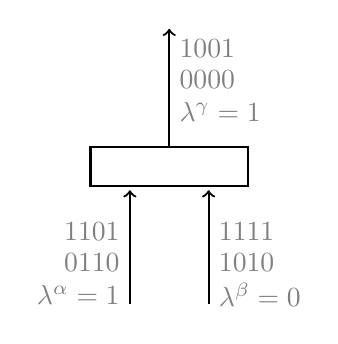
\begin{tikzpicture}[thick]
          \draw[black] (0,0) rectangle (2,0.5);
          \draw[->] (0.5,-1.5) -- 
          node[left,yshift=.2cm,opacity=.5]{1101} 
          node[left,yshift=-.2cm,opacity=.5]{0110}
          node[left,yshift=-.6cm,opacity=.5]{$\lambda^\alpha=1$} 
          (0.5,-.05);
          \draw[->] (1.5,-1.5) -- 
          node[right,yshift=.2cm,opacity=.5]{1111} 
          node[right,yshift=-.2cm,opacity=.5]{1010}
          node[right,yshift=-.6cm,opacity=.5]{$\lambda^\beta=0$} 
          (1.5,-.05);
          \draw[->] (1,.5) -- 
          node[right,yshift=.5cm,opacity=.5]{1001} 
          node[right,yshift=.1cm,opacity=.5]{0000}
          node[right,yshift=-.3cm,opacity=.5]{$\lambda^\gamma=1$} 
          (1,2);
        \end{tikzpicture}
      \end{center}
    \end{column}
    \begin{column}{.7\textwidth}
      \begin{eqnarray*}
        A^g_{10} 
        &=& G_0^*(s^\alpha_1) \oplus G_1^*(s^\beta_0) \oplus s_{[(\lambda^\alpha\oplus 1)\wedge(\lambda^\beta\oplus 0)]\oplus\lambda^\gamma}^\gamma \\[.2cm]
        &=& G_0^*(1101) \oplus G_1^*(1010) \oplus s_{[(1 \oplus 1)\wedge(0\oplus 0)]\oplus\lambda^\gamma}^\gamma \\[.2cm]
        % &=& G_b(s_{1,1}^\alpha)\oplus G_b(s_{1,2}^\alpha) \oplus G_b(s_{1,3}^\alpha) 
        % \ \oplus \  \\ 
        % & & G_a(s_{0,1}^\beta)\oplus G_a(s_{0,2}^\beta) \oplus G_a(s_{0,3}^\beta) 
        % \ \oplus \  \\ 
        % & & s_{[(\lambda^\alpha\oplus a) \wedge (\lambda^\beta\oplus b)]\oplus\lambda^\gamma}^\gamma \\
        &=& G_0(1)\oplus G_0(1) \oplus G_0(0) 
        \ \oplus \  \\ 
        & & G_1(1)\oplus G_1(0) \oplus G_1(1) 
        \ \oplus \  \\ 
        & & s_{[(1 \oplus 1)\wedge (0 \oplus 0)]\oplus 1}^\gamma \\[.2cm]
        &=& 1110 \oplus 1110 \oplus 0000
        \ \oplus \  \\ 
        & & 1111 \oplus 0001 \oplus 1111
        \ \oplus \  \\ 
        & & s_{[0 \wedge 0] \oplus 1}^\gamma \\[.25cm]
        &=& 0000 \oplus 0001 \oplus 1001 = 1000
      \end{eqnarray*}

    \end{column}
  \end{columns}
\end{frame}

\begin{frame}
  \frametitle{Gate labels -- ordinary gates}
  \note[item]{Next: Gate labels for splitters.}
  \begin{itemize}
  \item Gate labels for gate $g$:
    \begin{eqnarray*}
      A_{ab}^g &= & G_b(s_{a1}^\alpha)\oplus\dots\oplus G_b(s_{an}^\alpha) 
      \ \oplus \  \\ \nonumber
      & & G_a(s_{b1}^\beta)\oplus\dots\oplus G_a(s_{bn}^\beta)
      \ \oplus \ \\ \nonumber
      & & s_{[(\lambda^\alpha\oplus a)\otimes(\lambda^\beta\oplus b)]\oplus\lambda^\gamma}^\gamma
    \end{eqnarray*}
  \item Constant number of rounds, polynomial communication (constant-depth/bounded fan-in)
  \item %Pseudorandom generators one way $\Rightarrow$ 
    Signals $s_{ai}^\alpha$ and $s_{bj}^\beta$ cannot be deduced from the gate labels
  \item Neither can the semantics $\lambda^\alpha$, $\lambda^\beta$ and $\lambda^\beta$
  \end{itemize}
\end{frame}

\begin{frame}
  \frametitle{Gate labels -- splitter gates}
  \begin{itemize}
  \item Completely analogue to ordinary gates
  \item Incoming wire $\alpha$, outgoing wires $\gamma_0$, $\gamma_1$
    \begin{eqnarray*}
      A_{ab}^g & = & G_b(s^\alpha_{a1}) \oplus \dots \oplus G_b(s^\alpha_{an}) \oplus s^{\gamma_b}_{(\lambda^\alpha\oplus a)\oplus\lambda^{\gamma_b}}
    \end{eqnarray*}
  \item Again, compute gate labels for all combinations of $a$ and $b$
  \item Again computable in a constant number of rounds, polynomial communication
  \end{itemize}
\end{frame}

\section{Phase 2}
\label{sec:phase-2}

\subsection{Phase 2: Evaluating the Garbled Circuit}
\label{sec:phase-2-evaluation}

\begin{frame}
  \frametitle{Phase 2: evaluating the garbled circuit}
  \begin{itemize}
  \item Players computed:
    \begin{itemize}
    \item Garbled input signals
    \item Gate labels
    \end{itemize}
  \item Players \emph{individually} evaluate the garbled circuit gate by gate
  \item Compute gate output using gate labels
  \end{itemize}
  \note[item]{Next: ``The important part is how signals propagate along gates. That's what we will inspect now.''}
\end{frame}

\begin{frame}
  \frametitle{Evaluating an ordinary gate}
  \begin{itemize}
  \item Given: Garbled gate $g$ with signals $\sigma^\alpha$ and $\sigma^\beta$ along input wires $\alpha$ and $\beta$
  \item Input signals carry parity $a$ and $b$, respectively
  \item Reconsider equation (\ref{eqn:gate-labels-definition}): 

    \begin{equation*}
      A^g_{ab} = G_b^*(\sigma^\alpha_a) \oplus G_a^*(\sigma^\beta_b) \oplus \underbrace{\sigma_{[(\lambda^\alpha\oplus a)\otimes(\lambda^\beta\oplus b)]\oplus\lambda^\gamma}^\gamma}_{\text{Proper output}}
    \end{equation*}
  \item We can solve to obtain the output:

    \begin{equation*}
      \sigma^\gamma = G_b^*(\sigma^\alpha) \oplus G_a^*(\sigma^\beta) \oplus A_{ab}^g
    \end{equation*}
  \item Precise output computation:
    \begin{equation*}
      \sigma^\gamma=G_b(\sigma_1^{\alpha})\oplus\dots\oplus G_b(\sigma_n^{\alpha})
      \ \oplus \
      G_a(\sigma_1^{\beta})\oplus\dots\oplus G_a(\sigma_n^{\beta})
      \ \oplus\ 
      A_{ab}^g
    \end{equation*}

  \end{itemize}
\end{frame}

\begin{frame}
  \frametitle{Evaluating an ordinary gate -- example}
  Back to our previous example ($k=1$, $n=3$, $G_i(x)=x x x i$):

\begin{columns}
    \begin{column}{.3\textwidth}
      \begin{center}
        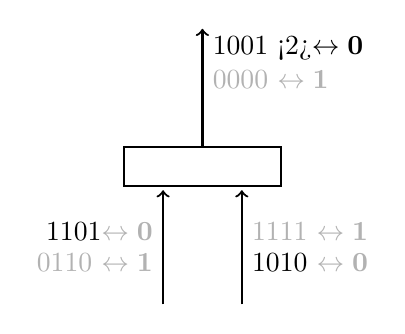
\begin{tikzpicture}[thick]
          \draw[black] (0,0) rectangle (2,0.5);
          \draw[->] (0.5,-1.5) -- 
          node[left,yshift=.2cm]{1101\color{black!30!white}{$\leftrightarrow \mathbf{0}$}} 
          node[left,yshift=-.2cm,opacity=.3]{0110 $\leftrightarrow \mathbf{1}$}
          %node[left,yshift=-.6cm]{$\lambda^\alpha=1$} 
          (0.5,-.05);
          \draw[->] (1.5,-1.5) -- 
          node[right,yshift=.2cm,opacity=.3]{1111 $\leftrightarrow \mathbf{1}$} 
          node[right,yshift=-.2cm]{1010 \color{black!30!white}{$\leftrightarrow \mathbf{0}$}}
          %node[right,yshift=-.6cm]{$\lambda^\beta=0$} 
          (1.5,-.05);
          \draw[->] (1,.5) -- 
          node[right,yshift=.5cm,onslide=<1>{opacity=.3},onslide=<2>{opacity=1}]{1001 \only<2>{\color{black!30!white}}{$\leftrightarrow \mathbf{0}$}} 
          node[right,yshift=.1cm,opacity=.3]{0000 $\leftrightarrow \mathbf{1}$}
          %node[right,yshift=-.3cm]{$\lambda^\gamma=1$} 
          (1,2);
        \end{tikzpicture}
      \end{center}
    \end{column}
    \begin{column}{.6\textwidth}
      \begin{itemize}
      \item Parities along $\alpha$ resp. $\beta$ are $a=1$ resp. $b=0$ $\Rightarrow$ use gate label $A^g_{10}=1000$ (computed before)
      \item Compute output: 
        \begin{eqnarray*}
          \sigma^\gamma &=& G_0^*(\sigma^\alpha_1) \oplus G_1^*(\sigma^\beta_0) \oplus A_{ab}^g \\[.25cm]
          &=& G_0^*(1101) \oplus G_1^*(1010) \oplus 1000 \\[.25cm]
          &=& 0000 \oplus 0001 \oplus 1000 = 1001
        \end{eqnarray*}

      \end{itemize}
    \end{column}
  \end{columns}
\end{frame}


\begin{frame}
  \frametitle{Evaluating a splitter gate}
  \begin{itemize}
  \item Completely analogue technique
  \item $\Rightarrow$ Outputs along wires $\gamma_0$, $\gamma_1$ for a splitter gate:
    \begin{equation*}
      \sigma^{\gamma_i}=G_i(\sigma_1^\alpha)\oplus\dots\oplus G_i(\sigma_n^\alpha) \ \oplus A_{ai}^g
    \end{equation*}
  \end{itemize}
\end{frame}

\section{Outcome}

\subsection{Outcome}
\label{sec:outcome}

\begin{frame}
  \frametitle{Outcome}
  \begin{itemize}
  \item Collaborative construction
    \begin{itemize}
    \item Constant number of rounds
    \item Polynomial communication amount
    \item Relies on existing sub-protocols
    \end{itemize}
  \item Local garbled circuit evaluation without collaboration
  \item Use of pseudorandom generators and splitters hides plain-text
  \end{itemize}
  Strength of the protocoll:
  \begin{itemize}
  \item Random signals and semantics
  \item Even if we know the parity-0-signal, we cannot deduce the proper parity-1-signal
  \item Independence of gate labels, signals and semantics
  \end{itemize}
\end{frame}

\part{Deferred or Omitted Explanations}
\label{part:deferred-explanations}

\section{Security Definition}

\subsection{Why wasn't that mentioned in detail?}

\begin{frame}
  \frametitle{Why I left it out}
  \begin{itemize}
  \item A whole bunch of technical definitions
  \item No groundbreaking insights
  \item ``Only'' needed for formal verification of the protocol
  \end{itemize}
\end{frame}

\subsection{Negligibility}
\label{sec:negligibility}

\begin{frame}
  \frametitle{Negligibility}
  \note[item] {Negligibility is one of the basic formal tools to describe security.}
  \begin{definition}[Negligibility]
    A function $\epsilon(k)$ is called \emph{negligible}, if for all $c>0$ there exists some $k_0$ such that $\epsilon(k) < k^{-c}$ for all $k>k_0$.
  \end{definition}
  \begin{itemize}
  \item In essence: Negligible if vanishing faster than any polynomial-inverse
  \item $k$ is usually the \emph{security parameter}
  \item In our case, $k$ will (in some way) bound the number of participants
  \item Example: If the probability is negligible, we simply say: ``That won't happen!''
  \end{itemize}
\end{frame}

\subsection{Strings and Ensembles}
\label{sec:strings-ensembles}

\begin{frame}
  \frametitle{Strings, ensembles}
  \begin{definition}
    Given some alphabet $\Sigma$, we denote the set of all
    (finite-length) strings by $\Sigma^*$.
  \end{definition}
  \begin{definition}[Ensemble]
    A family of probability measures $\left\{ {\cal A}_k\right\} $ on $\Sigma^*$ is called an ensemble, if only strings of length at most $q(k)$ have positive probability of being picked, where $q(k)$ is some polynomial in $k$.
  \end{definition}
\end{frame}

\subsection{Indistinguishability}

\begin{frame}
  \frametitle{Indistinguishability}
  \begin{definition}[Indistinguishability]
    For ${\cal A}$ taken from an ensemble and $C$ a boolean circuit, $p_{{\cal A}}^C$ is the probability that $C$ outputs 1 on an input randomly drawn according to distribution ${\cal A}$.

    Ensembles ${\cal A}$ and ${\cal B}$ \emph{computationally indistinguishable} if for any poly-size circuit family ${\cal C}=\left\{ C_k \right\}$, the function $\epsilon(k):=|p_{{\cal A}_k}^{{\cal C}_k}-p_{{\cal B}_k}^{{\cal C}_k}|$ is negligible.

    We call them \emph{statistically indistinguishable} if
    \begin{equation*}
      \epsilon(k):=\max_{S_k\subseteq \Sigma^*}|\Pr_{{\cal A}_k}[S_k]-\Pr_{{\cal B}_k}[S_k]|
    \end{equation*} is negligible, where $\Pr_{{\cal A}}[S]$ denotes the probability that we get a string within $S$ if we draw randomly according to ${\cal A}$.

  \end{definition}

\end{frame}

\subsection{Oracles}

\begin{frame}
  \frametitle{Notation: tagged vectors}
  \begin{itemize}
  \item Vectors $\overrightarrow{v}=(v_1,\dots,v_n)$ and $\overrightarrow{w}=(w_1,\dots,w_n)$
  \item $T\subseteq \left\{ 1,2,\dots,n \right\}$
  \item $\overrightarrow{v}_T := \left\{ (i,v_i) \mid i\in T \right\}$
  \item $\overline{T}=\left\{ 1,2,\dots,n \right\}\setminus T$
  \item $\overrightarrow{v}_T\cup \overrightarrow w_{\overline{T}}$ is the vector whose component indexed with indices from $T$ are taken from $\overrightarrow{v}$, all other components are taken from $\overrightarrow{w}$
  \end{itemize}
\end{frame}

\begin{frame}
  \frametitle{Oracles}
  \begin{definition}[$t$-bounded oracle]
    A $t$-bounded $(\overrightarrow{x},f)$-oracle is an oracle accepting two kinds of queries:
    \begin{itemize}
    \item Component query: A component query is an integer $i\in \{1,2,\dots,n\}$. If is only answered if $t$ or fewer component queries were made so far. If this is the case, the oracle distinguishes:
      \begin{itemize}
      \item If there was no output query so far, it is answered by $x_i$.
      \item If there was already a proper output query (see below), namely $\overrightarrow{x}'_T$, the query is answered by $(x_i,f_i(\overrightarrow{x}_{\overline{T}}\cup\overrightarrow{x}'_{T}))$.
      \end{itemize}
    \item Output query: An output query is a ``tagged vector'' $\overrightarrow{x}'_T$ (see below). It is answered by $f_T(\overrightarrow{x}_{\overline{T}}\cup\overrightarrow{x}'_{T})$ if $T$ consists precisely of the component queries made up to now and if there were not output queries so far. Further or improper output queries stay unanswered.
    \end{itemize}
  \end{definition}
\end{frame}

\subsection{Formal Definition of Security}

\begin{frame}
  \frametitle{Some probability spaces}
  \begin{itemize}
  \item Adverasry $A$'s knowledge defines a probability space: $\mathbf{VIEW}_A^k(\overrightarrow{x})$
  \item Output of uncorrupted players: $\mathbf{OUTPUT}_A^k(\overrightarrow{x})$
  \item Output of a random algorithm $S$ using an oracle: $\textsc{Output } S^{O_t(\overrightarrow{x},f)}(1^k)$
  \item $\textsc{Queries } S^{O_t(\overrightarrow{x},f)}(1^k)$ is a pair containing:

    \begin{itemize}
    \item The indices $i$ for which there was \emph{never} a component query.
    \item The (single) output query that was made by $S$.
    \end{itemize}

  \end{itemize}
\end{frame}

\begin{frame}
  \frametitle{Security}  
  \begin{definition}[Privacy, Correctness]
    Let $f:(\Sigma^l)^n\rightarrow(\Sigma^l)^n$. A protocol ${\cal P}$ $t$-securely computes $f$ if for all $t$-adversaries $A$ there exists a simulator $S$ (probably using a $t$-bounded oracle) such that the following hold:
    \begin{description}
    \item[Privacy] For all $\overrightarrow{x}\in(\Sigma^l)^n$, the $k$-parametrized ensemble $\mathbf{VIEW}_A^k(\overrightarrow{x})$ and the ensemble $\textsc{Output } S^{O_t(\overrightarrow{x},f)}(1^k)$ are computationally indistinguishable.
    \item[Correctness] For all $\overrightarrow{x}\in(\Sigma^l)^n$, the $k$-parametrized ensembles $\mathbf{OUTPUT}_A^k(\overrightarrow{x})$ and $[(G,\overrightarrow{x}'_T) \leftarrow \textsc{Queries } S^{O_t(\overrightarrow{x},f)}(1^k)\mid f_G(\overrightarrow{x}_{\overline{T}}\cup\overrightarrow{x}'_T)]$ are statistically indistinguishable.
    \end{description}
  \end{definition}

\end{frame}

\section{Protocol Security}

\subsection{General Idea}

\begin{frame}
  \frametitle{Proving the protocol secure}
  \begin{itemize}
  \item We did not concretely specify a sub-protocol that computes gate labels and garbled input signals \dots
  \item \dots but we said that appropriate sub-protocols \emph{exist}
  \item $\Rightarrow$ Quite a large amount of proof work is then done by the inventors of these sub-protocols
  \item Remaining proof constructs one simulator that works for \emph{all} adversaries
  \end{itemize}
  Today no detailed proof:
  \begin{itemize}
  \item Original proof (without splitters, thus not completely correct) spans twenty pages and twelve sub-proofs
  \item Additional work for splitters (done about ten years later) involves another very non-trivial proof
  \end{itemize}
\end{frame}

\section{Pseudorandom Generators}

\subsection{The Simple Answer}

\begin{frame}
  \frametitle{The need for pseudorandom generators}
  Why do we use them?
  \begin{itemize}
  \item Short answer: Because we need them!
  \item Long answer: No pseudorandom generators 

    $\Rightarrow$ operate directly on (garbled) signals
    
    i.e. $A_{ab}^g = s^\alpha_a \oplus s^\beta_b \oplus s^\gamma_{[(a\oplus\lambda^\alpha)\otimes(b\oplus\lambda^\beta)]\oplus\lambda^\gamma}$
  \item $\Rightarrow$ We could deduce the plain-text values.
  \end{itemize}
\end{frame}

\subsection{A Simple Attack without Pseudorandom Generators}

\begin{frame}
  \frametitle{A simple attack}
  \begin{itemize}
  \item Circuit $[(x \wedge y_1) \wedge y_2]$
  \item Assume I know that $x$ is $\mathbf{0}$
  \item $y_1, y_2$ supplied another party
  \item $\Rightarrow$ Global output represents \emph{surely} $\mathbf{0}$
  \item If there are no pseudorandom generators, we can deduce the plain-text of $y_2$
  \end{itemize}
  \begin{center}
    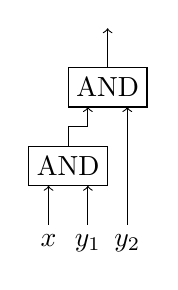
\begin{tikzpicture}
      \draw (0,0) rectangle (1,.5);
      \draw (0.5,1) rectangle (1.5,1.5);
      \draw[<-] (0.25, 0) -- +(0,-.5) node[below]{$x$};
      \draw[<-] (0.75, 0) -- +(0,-.5) node[below]{$y_1$};
      \draw[<-] (1.25, 1) -- +(0,-1.5) node[below]{$y_2$};
      \draw[->] (.5,.5) -- +(0,.25) -| (0.75, 1);
      \draw[->] (1,1.5) -- +(0,.5);
      \node at (.5,.25) {AND};
      \node at (1,1.25) {AND};
    \end{tikzpicture}
  \end{center}
\end{frame}

\begin{frame}
  \setbeamercovered{transparent}
  \frametitle{A simple attack -- first AND-gate}
  \begin{columns}
    \begin{column}{.75\textwidth}
      Our knowledge up to now (wlog):
      \begin{itemize}
      \item $s^\alpha_0\leftrightarrow \mathbf{0}$ (we said $x$ is 0)
      \item Signal along $\gamma$ has parity 0, and represents plain-text $\mathbf{0}$
      \item $\sigma^\gamma_{ab}$: signal along wire $\gamma$ for a parity-$a$-signal along $\alpha$ and a parity-$b$-signal along ${\beta_1}$
      \end{itemize}
      Now some calculations:
      \begin{itemize}
      \item<2-> $s_0^\gamma=A_{01}\oplus s_0^\alpha \oplus s_1^{\beta_1}$
      \item<4-> $\sigma_{10}^\gamma = A_{10} \oplus s_1^\alpha \oplus s_0^{\beta_1}$
      \item<4-> $\sigma_{11}^\gamma = A_{11} \oplus s_1^\alpha \oplus s_1^{\beta_1}$
      \item<4->$\Rightarrow \sigma_{10}^\gamma\oplus\sigma_{11}^\gamma = A_{10}\oplus A_{11} \oplus s_0^{\beta_1} \oplus s_1^{\beta_1}$
      \item<6->$\Rightarrow$ We know both signals and plain-text bits for $\gamma$
      \end{itemize}
    \end{column}
    \begin{column}{.25\textwidth}
      \begin{center}
        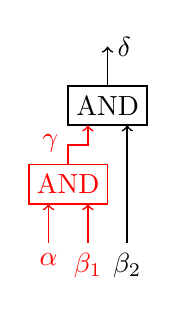
\begin{tikzpicture}[semithick]
          \draw[red] (0,0) rectangle (1,.5);
          \draw (0.5,1) rectangle (1.5,1.5);
          \draw[red,<-] (0.25, 0) -- +(0,-.5) node[below]{$\alpha$};
          \draw[red,<-] (0.75, 0) -- +(0,-.5) node[below]{${\beta}_1$};
          \draw[<-] (1.25, 1) -- +(0,-1.5) node[below]{${\beta}_2$};
          \draw[red,->] (.5,.5) -- node[left,yshift=.15cm]{$\gamma$} +(0,.25) -| (0.75, 1);
          \draw[->] (1,1.5) -- +(0,.5) node [right]{$\delta$};
          \node[red] at (.5,.25) {AND};
          \node at (1,1.25) {AND};
        \end{tikzpicture}
      \end{center}      
      Known values:

      \only<1->{$s_0^\alpha\leftrightarrow \mathbf{0}$}

      \vspace{.25cm}
      \only<1->{$s_0^{\beta_1}$} 
      \only<3->{$s_1^{\beta_1}$}

      \vspace{.25cm}
      \only<1->{$s_0^\gamma \leftrightarrow \mathbf{0}$}
      \only<5->{$s_1^\gamma \leftrightarrow \mathbf{1}$}
      
    \end{column}
  \end{columns}
\end{frame}

\begin{frame}
  \setbeamercovered{transparent}
  \frametitle{A simple attack -- second AND-gate}
  \begin{columns}
    \begin{column}{.75\textwidth}
      We know by now (wlog):
      \begin{itemize}
      \item $s^\gamma_0\leftrightarrow \mathbf{0}, s^\gamma_1\leftrightarrow \mathbf{1}$ (signals and plain-text association)
      \item $s_0^{\beta_2}$ (input signal for plain-text bit of other player)
      \item Gate labels $B_{00},B_{01},B_{10},B_{11}$
      \end{itemize}
      We compute $s_1^{\beta_2}$:
      \begin{itemize}
      \item<2-> $\sigma_{00}^\delta = B_{00} \oplus s_0^\gamma \oplus s_0^{\beta_2} \leftrightarrow \mathbf{0}$
      \item<2-> $\sigma_{01}^\delta = B_{01} \oplus s_0^\gamma \oplus s_1^{\beta_2} \leftrightarrow \mathbf{0}$
      \item<3->{$\Rightarrow$ Solve for $s_1^{\beta_2}$, and ``test gate'' with $s_1^\gamma$ and $\{ s_0^{\beta_2}, s_1^{\beta_2} \}$}
      \end{itemize}
    \end{column}
    \begin{column}{.25\textwidth}
      \begin{center}
        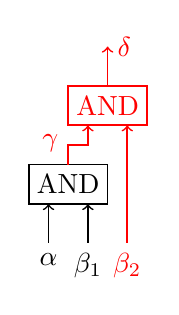
\begin{tikzpicture}[semithick]
          \draw (0,0) rectangle (1,.5);
          \draw[red] (0.5,1) rectangle (1.5,1.5);
          \draw[<-] (0.25, 0) -- +(0,-.5) node[below]{$\alpha$};
          \draw[<-] (0.75, 0) -- +(0,-.5) node[below]{$\beta_1$};
          \draw[red,<-] (1.25, 1) -- +(0,-1.5) node[below]{$\beta_2$};
          \draw[red,->] (.5,.5) -- node[left,yshift=.15cm]{$\gamma$} +(0,.25) -| (0.75, 1);
          \draw[red,->] (1,1.5) -- +(0,.5) node [right]{$\delta$};;
          \node at (.5,.25) {AND};
          \node[red] at (1,1.25) {AND};
        \end{tikzpicture}
      \end{center}      
    \end{column}
  \end{columns}
\end{frame}

% \begin{frame}
%   \frametitle{A simple attack -- the details}
%   \begin{itemize}
%   \item AND-gate with known gate labels $A_{ab}$
%   \item I supply $s_0^\alpha \leftrightarrow \mathbf{0}$ with parity 0
%   \item Other input is $s_0^\beta$ with parity $0$, plain-text shall stay private
%   \item I know: 

%     \begin{eqnarray*}
%       \sigma^\gamma & = & A_{00}^g\oplus s_0^\alpha \oplus s_0^\beta \stackrel{!}{\leftrightarrow} \mathbf{0} \\
%       \sigma^\gamma & = & A_{01}^g\oplus s_0^\alpha \oplus s_1^\beta \stackrel{!}{\leftrightarrow} \mathbf{0} \\
%       \Rightarrow s_1^\beta & = & A_{01}^g\oplus s_0^\alpha \oplus \sigma^\gamma \\
%       \Rightarrow s_1^\alpha & = & A_{11}^g \oplus s_1^\beta \
%     \end{eqnarray*}


%   \item $\Rightarrow$ Output of AND-gate represents \emph{surely} $\mathbf{0}$
%   \item All gate labels known

%     $\Rightarrow$ We can reconstruct all signals for the other wire

%     $\Rightarrow$ We can now compute all the signals for our wire

%     $\Rightarrow$ We now test all signal combinations and deduce values!
%   \end{itemize}
% \end{frame}

\begin{frame}
  \frametitle{How do pseudorandom generators help?}
  Without pseudorandom generators:
  \begin{itemize}
  \item Plain-text values computable
  \end{itemize}
  With pseudorandom generators:
  \begin{itemize}
  \item We can deduce the values $G_a^*(\sigma^\beta)$ \dots
  \item \dots but \emph{not} the values $\sigma^\beta$
  \item $\Rightarrow$ We do not know the proper other signal for wire $\beta$
  \item $\Rightarrow$ We cannot try all signal combinations
  \end{itemize}
  \begin{alertblock}{Essence:}
    Applying a pseudorandom generator onto the signals prevents us from deducing the proper signal for the complementary parity\footnote{And thus, from deducing plain-text values.}!
  \end{alertblock}
\end{frame}

\section{Splitters}

\subsection{Why do we need Splitters?}

\begin{frame}
  \frametitle{Why do we need splitters?}
  \begin{itemize}
  \item Without splitters, different gates are dependent
  \item $\Rightarrow$ This enables us to determine plain-text bits with high probability
  \end{itemize}
\end{frame}

\subsection{An Attack on Splitter-free Circuits}

\begin{frame}
  \frametitle{An attack on splitter-free circuits}
  A comparator for two $l$-bit numbers:
  \begin{center}
    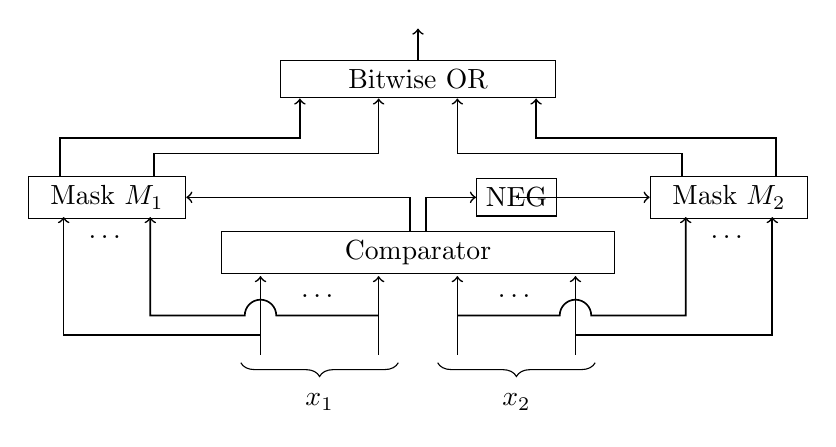
\begin{tikzpicture}
      \begin{scope}
        \draw[->,semithick] (-.25,-.50) -- (-.25,.5);
        \node at (.5,.25) {\dots};
        \draw[->,semithick] (1.25,-.50) -- (1.25,.5);
        \draw[decorate,decoration={brace,amplitude=0.5em}](1.5,-.6) -- (-.5,-.6);
        \node at (.5,-1.1) {$x_1$};
      \end{scope}
      \begin{scope}[xshift=2.5cm]
        \draw[->,semithick] (-.25,-.50) -- (-.25,.5); 
        \node at (.5,.25) {\dots}; 
        \draw[->,semithick] (1.25,-.50) -- (1.25,.5);
        \draw[decorate,decoration={brace,amplitude=0.5em}] (1.5,-.6) -- (-.5,-.6);
        \node at (.5,-1.1) {$x_2$};
      \end{scope}
      \node[shape=rectangle,minimum width=5cm,draw=black] (compi) at (1.75,.8) {Comparator};
      % x -> mask 1
      \draw[->,semithick] (-.25,-.25) -| +(-2.5,1.5);
      \node at (-2.2,1) {\dots};
      \draw[->,semithick] (1.25,0) -- ++(-1.3,0) arc(0:180:.2) -| +(-1.2,1.25);
      \node[shape=rectangle,draw=black,minimum width=2cm] (m1) at (-2.2,1.5) {Mask $M_1$};
      % y -> mask 2
      \begin{scope}[xshift=3.5cm,xscale=-1]
        \draw[->,semithick] (-.25,-.25) -| +(-2.5,1.5);
        \node at (-2.2,1) {\dots};
        \draw[->,semithick] (1.25,0) -- ++(-1.3,0) arc(0:180:.2) -| +(-1.2,1.25);+
        \node[shape=rectangle,draw=black] (neg) at (.5,1.5) {NEG};
        \node[shape=rectangle,draw=black,minimum width=2cm] (m2) at (-2.2,1.5) {Mask $M_2$};
      \end{scope}
      \draw[->,semithick] (compi.north)  +(-.1,0) |- (m1);
      \draw[->,semithick] (compi.north)  +( .1,0) |- (neg);    
      \draw[->,semithick] (neg) |- (m2);
      \node[shape=rectangle,draw=black,minimum width=3.5cm] (bo) at (1.75,3) {Bitwise OR};
      \coordinate[xshift=-.6cm] (m11) at (m1.north);
      \coordinate[xshift=.6cm] (m12) at (m1.north);
      \coordinate[xshift=-.6cm] (m21) at (m2.north);
      \coordinate[xshift=.6cm] (m22) at (m2.north);
      \draw[<-,semithick] (bo.south) +(-1.5,0) -- +(-1.5,-.5) -| (m11);
      \draw[<-,semithick] (bo.south) +(-0.5,0) -- +(-0.5,-.7) -| (m12);
      \draw[<-,semithick] (bo.south) +( .5,0) -- +( .5,-.7) -| (m21);
      \draw[<-,semithick] (bo.south) +(1.5,0) -- +(1.5,-.5) -| (m22);
      \draw[->,semithick] (bo.north) -- +(0,.4);
    \end{tikzpicture}
  \end{center}
  \begin{itemize}
  \item We assume that an earlier execution yielded $x_2\geq x_1$
  \item How can player 2 exploit this?
  \item $\Rightarrow$ Important part: Mask $M_1$
  \end{itemize}
\end{frame}

\begin{frame}
  \frametitle{An attack on splitter-free circuits} 
  \begin{center}
    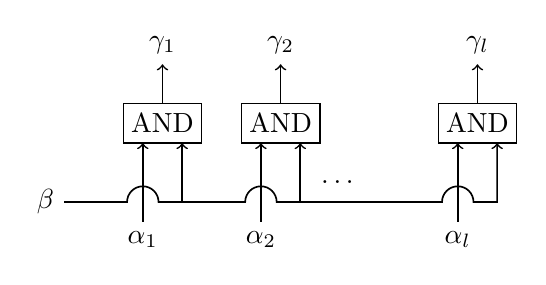
\begin{tikzpicture}
      \draw[->,semithick] (0,0) node[below]{$\alpha_{1}$} -- (0,1);
      \draw[->,semithick] (1.5,0) node[below]{$\alpha_{2}$} -- (1.5,1);
      \node at (2.5,.5) {\dots};
      \draw[->,semithick] (4,0) node[below]{$\alpha_{l}$} -- (4,1);
      \draw[->,semithick] (-1,.25) node[left] {$\beta$} -- (-.2,.25) arc(180:0:0.2) 
      -- (1.3,.25) arc(180:0:0.2) 
      -- (3.8,.25) arc(180:0:0.2) 
      -- (4.5,.25) -- (4.5,1);
      \draw[->,semithick] (.5,.25) -- (.5,1);
      \draw[->,semithick] (2,.25) -- (2,1);
      \draw(-.25,1)rectangle(.75,1.5);
      \draw(1.25,1)rectangle(2.25,1.5);
      \draw(3.75,1)rectangle(4.75,1.5);
      \draw[->,semithick](0.25,1.5) -- +(0,.5) node[above]{$\gamma_1$};
      \draw[->,semithick](1.75,1.5) -- +(0,.5) node[above]{$\gamma_2$};
      \draw[->,semithick](4.25,1.5) -- +(0,.5) node[above]{$\gamma_l$};
      \node at (0.25,1.25) {AND};
      \node at (1.75,1.25) {AND};
      \node at (4.25,1.25) {AND};
    \end{tikzpicture}
  \end{center}
  \begin{itemize}
  \item What would happen if $x_1$ was 0?
  \item Assume signals along $\alpha_i$ represents $\mathbf{0}$
  \item Assume that signal along $\beta$ represents $\mathbf{1}$
  \item We are able to deduce the correct values of $x_1$ with high probability
  \item This can be acchieved a probabilistic algorithm
  \end{itemize}
\end{frame}

\begin{frame}
  \frametitle{An attack on splitter-free circuits} 
  \begin{center}
    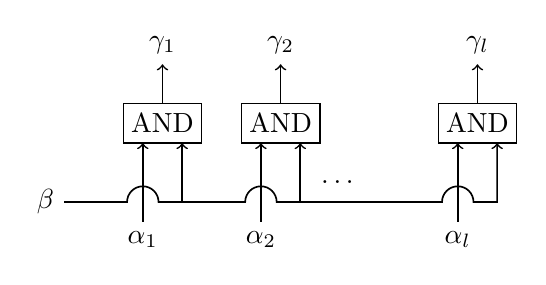
\begin{tikzpicture}
      \draw[->,semithick] (0,0) node[below]{$\alpha_{1}$} -- (0,1);
      \draw[->,semithick] (1.5,0) node[below]{$\alpha_{2}$} -- (1.5,1);
      \node at (2.5,.5) {\dots};
      \draw[->,semithick] (4,0) node[below]{$\alpha_{l}$} -- (4,1);
      \draw[->,semithick] (-1,.25) node[left] {$\beta$} -- (-.2,.25) arc(180:0:0.2) 
      -- (1.3,.25) arc(180:0:0.2) 
      -- (3.8,.25) arc(180:0:0.2) 
      -- (4.5,.25) -- (4.5,1);
      \draw[->,semithick] (.5,.25) -- (.5,1);
      \draw[->,semithick] (2,.25) -- (2,1);
      \draw(-.25,1)rectangle(.75,1.5);
      \draw(1.25,1)rectangle(2.25,1.5);
      \draw(3.75,1)rectangle(4.75,1.5);
      \draw[->,semithick](0.25,1.5) -- +(0,.5) node[above]{$\gamma_1$};
      \draw[->,semithick](1.75,1.5) -- +(0,.5) node[above]{$\gamma_2$};
      \draw[->,semithick](4.25,1.5) -- +(0,.5) node[above]{$\gamma_l$};
      \node at (0.25,1.25) {AND};
      \node at (1.75,1.25) {AND};
      \node at (4.25,1.25) {AND};
    \end{tikzpicture}
  \end{center}
  \begin{itemize}
  \item Assume that $\sigma^{\alpha_i}\leftrightarrow \mathbf{0}$ for all $i\in\{1,2,\dots,l\}$ (likely wrong)
  \item We know that $\sigma^{\gamma_i}\leftrightarrow \mathbf{0}$
  \item Idea: For all correctly-guessed bits, we get ``useful results'', for the wrongly-guessed bits, we obtian random stuff.
  \item Gate $i$:
    \begin{equation*}
        \sigma^{\gamma_i} = A^i_{ab} \oplus \underbrace{G^*_b(\sigma^{\alpha_i}_{a_i})}_{G_b(\sigma^{\alpha_i}_{a_i,1}) \oplus G_b(\sigma^{\alpha_i}_{a_i,2})} \oplus \underbrace{G^*_{a_i}(\sigma^\beta_b)}_{G_{a_i}(\sigma^\beta_{b,1}) \oplus G_{a_i}(\sigma^\beta_{b,2})}
    \end{equation*}
  \item $G^*_b(\sigma^{\alpha_i}_{a_i})$ present in \emph{all} gates
  \end{itemize}
\end{frame}

\begin{frame}
  \frametitle{An attack on splitter-free circuits}
  \begin{itemize}
  \item Gate $i$:
    \begin{equation*}
        \sigma^{\gamma_i} = A^i_{ab} \oplus \underbrace{G^*_b(\sigma^{\alpha_i}_{a_i})}_{G_b(\sigma^{\alpha_i}_{a_i,1}) \oplus G_b(\sigma^{\alpha_i}_{a_i,2})} \oplus \underbrace{G^*_{a_i}(\sigma^\beta_b)}_{G_{a_i}(\sigma^\beta_{b,1}) \oplus G_{a_i}(\sigma^\beta_{b,2})}
    \end{equation*}
  \item $G^*_{a_i}(\sigma^{\beta}_{b})$ present in \emph{all} gates
  \item ``Solve'' for $G^*_{a_i}(\sigma^\beta_b)$ and rename result:
    \begin{equation*}
        \mu_i:=\sigma^{\gamma_i}\oplus G_b(s^{\alpha_i}_{a,1}) \oplus G_b(s^{\alpha_i}_{a,2}) \oplus A^{g_i}_{a_i b}
    \end{equation*}
  \item If our guess for bit $i$ was correct, $\mu_i$ corresponds to $G^*_{a_i}(\sigma^\beta_b)$, otherwise it is a random string
  \end{itemize}
\end{frame}

\begin{frame}
  \frametitle{An attack on splitter-free circuits}
  \begin{itemize}
  \item Collection of $\mu_i$'s
  \item Correct guesses:

    $\Rightarrow$ either $G_0(s^\beta_{b1})\oplus G_0(s^\beta_{b2})$ or $G_1(s^\beta_{b1})\oplus G_1(s^\beta_{b2})$
  \item Incorrect guesses: Random strings
  \item $\Rightarrow$ group the $\mu_i$'s (random vs. $G_0(s^\beta_{b1})\oplus G_0(s^\beta_{b2})$ or $G_1(s^\beta_{b1})\oplus G_1(s^\beta_{b2})$)
  \item $\Rightarrow$ random strings correspond to wrongly-guessed bits $\Rightarrow$ these bits are probably $\mathbf{1}$, all the others are probably $\mathbf{0}$
  \end{itemize}
\end{frame}

\part{Literature}
\label{part:literature}

\section{Literature}
\label{sec:literature}

\begin{frame}
  \frametitle{For further reading: original protocol description}
  \begin{thebibliography}{10}

  \bibitem{Rogaway:1991:RCS:888502}
    Rogaway, P.:
    \newblock {The Round Complexity Of Secure Protocols}.
    \newblock Technical report, Massachusetts Institute of Technology, Cambridge,
    MA, USA (1991)

  \bibitem{Beaver1990}
    Beaver, D., Micali, S., Rogaway, P.:
    \newblock {The round complexity of secure protocols}.
    \newblock In: Proceedings of the twenty-second annual ACM symposium on Theory
    of computing, New York, NY, USA, ACM (1990)  503--513

  \end{thebibliography}

\end{frame}

\begin{frame}
  \frametitle{For further reading: splitter construction}
  \begin{thebibliography}{10}
  \bibitem{Tate03ongarbled}
    Tate, S.R., Xu, K.:
    \newblock {On Garbled Circuits and Constant Round Secure Function Evaluation}.
    \newblock Technical report, UNIVERSITY OF NORTH TEXAS (2003)

  \bibitem{Xu:2004:MAS:1023552}
    Xu, K.:
    \newblock Mobile agent security through multi-agent cryptographic protocols.
    \newblock PhD thesis, University of North Texas, Denton, TX, USA (2004)
    AAI3126591.    
  \end{thebibliography}
\end{frame}

\begin{frame}
  \frametitle{For further reading: a modern treatment of garbled circuits}
  \begin{thebibliography}{10}
  \bibitem{bellare-hoang-rogaway-garbling-schemes}
    Bellare, M., Hoang, V.T., Rogaway, P.:
    \newblock Garbling schemes.
    \newblock Cryptology ePrint Archive, Report 2012/265 (2012)
    \url{http://eprint.iacr.org/}.
  \end{thebibliography}
\end{frame}

\begin{frame}
  \frametitle{For further reading: general crypto readings}  
  \begin{thebibliography}{10}
  \bibitem{lecture-notes-goldwasser-bellare}
    Goldwasser, S., Bellare, M.:
    \newblock Lecture notes on cryptography.
    \newblock Lecture Notes (July 2008) Accessed March 2012
    (\url{http://cseweb.ucsd.edu/users/mihir/papers/gb.pdf}).

  \bibitem{goldreich_foundations_of_crypto_2}
    Goldreich, O.:
    \newblock Foundations of Cryptography: Volume 2, Basic Applications.
    \newblock Cambridge University Press, New York, NY, USA (2004)
  \end{thebibliography}
\end{frame}

\begin{frame}
  \frametitle{For further reading: pseudorandom generators and one-way functions}
  \begin{thebibliography}{10}
  \bibitem{pseudorandom-generators-blum}
    Blum, M., Micali, S.:
    \newblock How to generate cryptographically strong sequences of pseudo-random
    bits.
    \newblock SIAM J. Comput. \textbf{13}(4) (November 1984)  850--864

  \bibitem{yao-theory-application-trapdoor-functions}
    Yao, A.C.:
    \newblock Theory and application of trapdoor functions.
    \newblock In: Proceedings of the 23rd Annual Symposium on Foundations of
    Computer Science. SFCS '82, Washington, DC, USA, IEEE Computer Society (1982)
    80--91
  \end{thebibliography}
\end{frame}

\begin{frame}[allowframebreaks]
  \frametitle{For further reading: other readings}
  \begin{thebibliography}{10}
  \bibitem{shamir_secret_sharing}
    Shamir, A.:
    \newblock How to share a secret.
    \newblock Commun. ACM \textbf{22}(11) (November 1979)  612--613

  \bibitem{verifiable-secret-sharing-chor-ben-gold-sha-mic}
    Chor, B., Goldwasser, S., Micali, S., Awerbuch, B.:
    \newblock Verifiable secret sharing and achieving simultaneity in the presence
    of faults.
    \newblock In: Proceedings of the 26th Annual Symposium on Foundations of
    Computer Science. SFCS '85, Washington, DC, USA, IEEE Computer Society (1985)
    383--395

  \bibitem{rabin-ben-or-verifiable-secret-sharing-number-rounds}
    Rabin, T., Ben-Or, M.:
    \newblock Verifiable secret sharing and multiparty protocols with honest
    majority.
    \newblock In: Proceedings of the twenty-first annual ACM symposium on Theory of
    computing. STOC '89, New York, NY, USA, ACM (1989)  73--85

  \bibitem{beaver-verifiable-secret-sharing}
    Beaver, D.:
    \newblock Multiparty protocols tolerating half faulty processors.
    \newblock In: Proceedings on Advances in cryptology. CRYPTO '89, New York, NY,
    USA, Springer-Verlag New York, Inc. (1989)  560--572

  \bibitem{how-to-play-any-mental-game-goldreich-micali-wigderson}
    Goldreich, O., Micali, S., Wigderson, A.:
    \newblock How to play any mental game.
    \newblock In: Proceedings of the nineteenth annual ACM symposium on Theory of
    computing. STOC '87, New York, NY, USA, ACM (1987)  218--229

  \bibitem{completeness-theorems-non-crypto-fault-tolerant}
    Ben-Or, M., Goldwasser, S., Wigderson, A.:
    \newblock Completeness theorems for non-cryptographic fault-tolerant
    distributed computation.
    \newblock In: Proceedings of the twentieth annual ACM symposium on Theory of
    computing. STOC '88, New York, NY, USA, ACM (1988)  1--10
  \end{thebibliography}
\end{frame}

\end{document}

%%% Local Variables: 
%%% mode: latex
%%% TeX-master: t
%%% End: 
